\chapter{Physik}
\section{11.12.2008}
\subsection{11.12.2008-IMG-phys-1}
\begin{tikzpicture}
	\draw[thick] (0,0) node [left] {$G$} -- (2,0);
	\draw[thick] (0,0) circle (0.07);
	\draw[thick] (2,1) -- (2,-1);

	\draw[thick] (3,1) -- (3,-1);

	\draw[thick] (3,1) -- (4,1) -- (4,3) node [right] {$D$};
	\draw[thick] (4,3) circle (0.07);

	\draw[thick] (3,-1) -- (4,-1) -- (4,-3) node [right] {$S$};
	\draw[thick] (4,-3) circle (0.07);

	\draw[thick] (3,0) -- (5,0) node [right] {$B$};
	\draw[thick] (5,0) circle (0.07);
\end{tikzpicture}
\begin{lstlisting}[frame=single]
\end{lstlisting}
\begin{tikzpicture}
	\draw[thick] (0,0) node [left] {$G$} -- (2,0);
	\draw[thick] (0,0) circle (0.07);
	\draw[thick] (2,1) -- (2,-1);

	\draw[thick] (3,1) -- (3,-1);

	\draw[thick] (3,1) -- (4,1) -- (4,3) node [right] {$D$};
	\draw[thick] (4,3) circle (0.07);

	\draw[thick] (3,-1) -- (4,-1) -- (4,-3) node [right] {$S$};
	\draw[thick] (4,-3) circle (0.07);

	\draw[thick] (3,0) -- (5,0) node [right] {$B$};
	\draw[thick] (5,0) circle (0.07);
\end{tikzpicture}


\subsection{11.12.2008-IMG-phys-3}
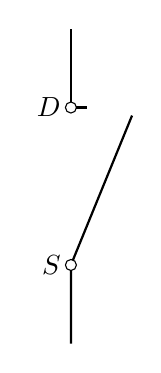
\begin{tikzpicture}
	\draw[thick] (0,0) -- (0,1) node [left] {$S$} -- (75:3);
	\draw[thick] (0.2,3) -- (0,3) node [left] {$D$} -- (0,4);

	\draw[fill=white] (0,1) circle (0.07);
	\draw[fill=white] (0,3) circle (0.07);
\end{tikzpicture}
\begin{lstlisting}[frame=single]
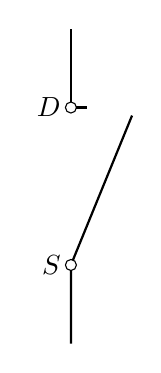
\begin{tikzpicture}
	\draw[thick] (0,0) -- (0,1) node [left] {$S$} -- (75:3);
	\draw[thick] (0.2,3) -- (0,3) node [left] {$D$} -- (0,4);

	\draw[fill=white] (0,1) circle (0.07);
	\draw[fill=white] (0,3) circle (0.07);
\end{tikzpicture}
\end{lstlisting}

\subsection{11.12.2008-IMG-phys-4}
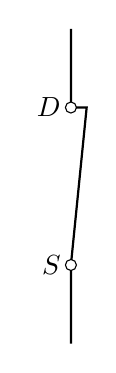
\begin{tikzpicture}
	\draw[thick] (0,0) -- (0,1) node [left] {$S$} -- (0.2,3) -- (0,3) node [left] {$D$} -- (0,4);

	\draw[fill=white] (0,1) circle (0.07);
	\draw[fill=white] (0,3) circle (0.07);
\end{tikzpicture}
\begin{lstlisting}[frame=single]
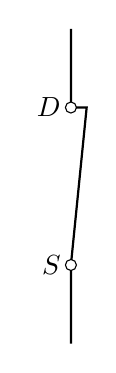
\begin{tikzpicture}
	\draw[thick] (0,0) -- (0,1) node [left] {$S$} -- (0.2,3) -- (0,3) node [left] {$D$} -- (0,4);

	\draw[fill=white] (0,1) circle (0.07);
	\draw[fill=white] (0,3) circle (0.07);
\end{tikzpicture}
\end{lstlisting}

\subsection{11.12.2008-IMG-phys-6}
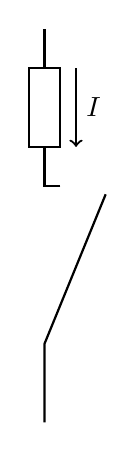
\begin{tikzpicture}
	\draw[thick] (0,0) -- (0,1) -- (75:3);
	\draw[thick] (0.2,3) -- (0,3) -- (0,5);

	\draw[thick, fill=white] (-0.2,3.5) rectangle (0.2,4.5);

	\draw[->, thick] (0.4,4.5) -- (0.4,3.5) node [midway, right] {$I$};
\end{tikzpicture}
\begin{lstlisting}[frame=single]
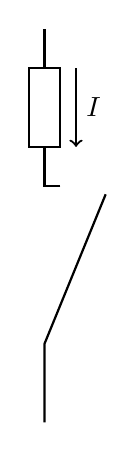
\begin{tikzpicture}
	\draw[thick] (0,0) -- (0,1) -- (75:3);
	\draw[thick] (0.2,3) -- (0,3) -- (0,5);

	\draw[thick, fill=white] (-0.2,3.5) rectangle (0.2,4.5);

	\draw[->, thick] (0.4,4.5) -- (0.4,3.5) node [midway, right] {$I$};
\end{tikzpicture}
\end{lstlisting}

\subsection{11.12.2008-IMG-phys-7}
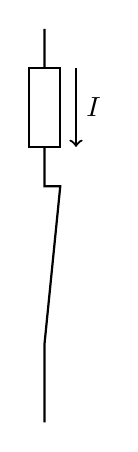
\begin{tikzpicture}
	\draw[thick] (0,0) -- (0,1) -- (0.2,3) -- (0,3) -- (0,5);

	\draw[thick, fill=white] (-0.2,3.5) rectangle (0.2,4.5);

	\draw[->, thick] (0.4,4.5) -- (0.4,3.5) node [midway, right] {$I$};
\end{tikzpicture}
\begin{lstlisting}[frame=single]
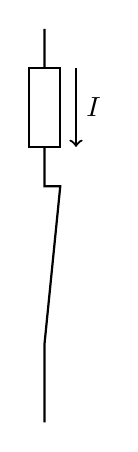
\begin{tikzpicture}
	\draw[thick] (0,0) -- (0,1) -- (0.2,3) -- (0,3) -- (0,5);

	\draw[thick, fill=white] (-0.2,3.5) rectangle (0.2,4.5);

	\draw[->, thick] (0.4,4.5) -- (0.4,3.5) node [midway, right] {$I$};
\end{tikzpicture}
\end{lstlisting}

\section{22.12.2008}
\subsection{22.12.2008-IMG-phys-1}
\begin{tikzpicture}
	\draw[thick, ->] (0,-0.5) -- (0,6) node[left] {$z$};
	\draw[thick, ->] (-0.5,0) -- (8,0) node[below] {$x$};
	\draw[thick, ->] (-0.25,-0.25) -- (4,4) node[right] {$y$};

	\draw[draw=green, ->] (0,0) -- (4.5,-0.5);
	\draw[draw=blue, ->] (0,0) -- (2.5,1.5);
	\draw[draw=red, ->] (0,0) -- (0.5,3);

	\fill[green] (0,0) circle (3pt);
\end{tikzpicture}
\begin{lstlisting}[frame=single]
\begin{tikzpicture}
	\draw[thick, ->] (0,-0.5) -- (0,6) node[left] {$z$};
	\draw[thick, ->] (-0.5,0) -- (8,0) node[below] {$x$};
	\draw[thick, ->] (-0.25,-0.25) -- (4,4) node[right] {$y$};

	\draw[draw=green, ->] (0,0) -- (4.5,-0.5);
	\draw[draw=blue, ->] (0,0) -- (2.5,1.5);
	\draw[draw=red, ->] (0,0) -- (0.5,3);

	\fill[green] (0,0) circle (3pt);
\end{tikzpicture}
\end{lstlisting}

\subsection{22.12.2008-IMG-phys-2}
\begin{tikzpicture}
	\draw[thick, draw=blue, ->] (0,0) -- (0,-7);
	\draw[thick, draw=blue, ->] (2,0) -- (2,-7);
	\draw[thick, draw=blue, ->] (4,0) -- (4,-7);
\end{tikzpicture}
\begin{lstlisting}[frame=single]
\begin{tikzpicture}
	\draw[thick, draw=blue, ->] (0,0) -- (0,-7);
	\draw[thick, draw=blue, ->] (2,0) -- (2,-7);
	\draw[thick, draw=blue, ->] (4,0) -- (4,-7);
\end{tikzpicture}
\end{lstlisting}

\subsection{22.12.2008-IMG-phys-5}
\begin{tikzpicture}
	\draw[thick, dashed, draw=blue] (0,0) rectangle (9,7);
	\draw[thick, draw=blue] (1,1) node[text=blue] {$\times$} circle (0.25);
	\draw[thick, draw=blue] (8,1) node[text=blue] {$\times$} circle (0.25);
	\draw[thick, draw=blue] (1,6) node[text=blue] {$\times$} circle (0.25);
	\draw[thick, draw=blue] (8,6) node[text=blue] {$\times$} circle (0.25);
	\node[text=blue, above] at (4.5,7) {\LARGE{$\vec{B}$}};

	\draw[thick, draw=green!50!black, ->] (-3,5) -- (0,5) node[below, midway, text=green!50!black] {$e^-$-Strahl};
	\draw[thick, draw=green!50!black, dashed] (0,5) -- (4,5);

	\draw[thick] (4,3) circle (2);
	\fill (4,3) circle (1pt);
	\draw[thick, ->] (4,3) -- +(45:2) node[midway, below] {$r$};

	\draw[thick, draw=red, ->] (4,5) -- +(0,-1) node[text=red, left, midway] {$\vec{F_L}$};
	\draw[thick, draw=green!50!black, ->] (4,5) -- +(1,0) node[text=green!50!black, above, midway] {$\vec{v}$};
	\draw[thick, draw=green!50!black, fill=white] (4,5) node[text=green!50!black] {-} circle (3pt);

	\draw[thick, draw=green!50!black, ->] (6,3) -- +(0,-1) node[text=green!50!black, left, midway] {$\vec{v}$};
	\draw[thick, draw=red, ->] (6,3) -- +(-1,0) node[text=red, above, midway] {$\vec{F_L}$};
	\draw[thick, draw=green!50!black, fill=white] (6,3) node[text=green!50!black] {-} circle (3pt);
\end{tikzpicture}
\begin{lstlisting}[frame=single]
\begin{tikzpicture}
	\draw[thick, dashed, draw=blue] (0,0) rectangle (9,7);
	\draw[thick, draw=blue] (1,1) node[text=blue] {$\times$} circle (0.25);
	\draw[thick, draw=blue] (8,1) node[text=blue] {$\times$} circle (0.25);
	\draw[thick, draw=blue] (1,6) node[text=blue] {$\times$} circle (0.25);
	\draw[thick, draw=blue] (8,6) node[text=blue] {$\times$} circle (0.25);
	\node[text=blue, above] at (4.5,7) {\LARGE{$\vec{B}$}};

	\draw[thick, draw=green!50!black, ->] (-3,5) -- (0,5) node[below, midway, text=green!50!black] {$e^-$-Strahl};
	\draw[thick, draw=green!50!black, dashed] (0,5) -- (4,5);

	\draw[thick] (4,3) circle (2);
	\fill (4,3) circle (1pt);
	\draw[thick, ->] (4,3) -- +(45:2) node[midway, below] {$r$};

	\draw[thick, draw=red, ->] (4,5) -- +(0,-1) node[text=red, left, midway] {$\vec{F_L}$};
	\draw[thick, draw=green!50!black, ->] (4,5) -- +(1,0) node[text=green!50!black, above, midway] {$\vec{v}$};
	\draw[thick, draw=green!50!black, fill=white] (4,5) node[text=green!50!black] {-} circle (3pt);

	\draw[thick, draw=green!50!black, ->] (6,3) -- +(0,-1) node[text=green!50!black, left, midway] {$\vec{v}$};
	\draw[thick, draw=red, ->] (6,3) -- +(-1,0) node[text=red, above, midway] {$\vec{F_L}$};
	\draw[thick, draw=green!50!black, fill=white] (6,3) node[text=green!50!black] {-} circle (3pt);
\end{tikzpicture}
\end{lstlisting}

\subsection{22.12.2008-IMG-phys-3}
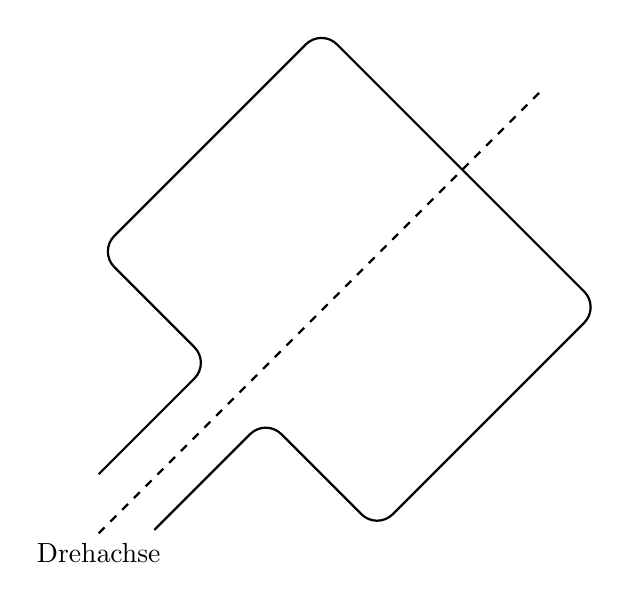
\begin{tikzpicture}
	\draw[thick,rounded corners=8pt] (0,0) -- ++(45:2) -- ++(135:2) -- ++(45:4) -- ++(-45:5) -- ++(-135:4) -- ++(135:2) -- ++(-135:2);
	\draw[thick, dashed] (0,-0.75) node[below] {Drehachse} -- +(45:8);
\end{tikzpicture}
\begin{lstlisting}[frame=single]
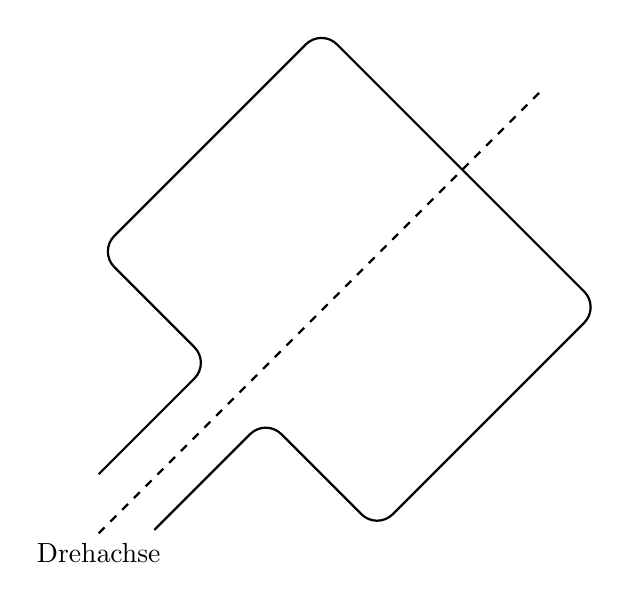
\begin{tikzpicture}
	\draw[thick,rounded corners=8pt] (0,0) -- ++(45:2) -- ++(135:2) -- ++(45:4) -- ++(-45:5) -- ++(-135:4) -- ++(135:2) -- ++(-135:2);
	\draw[thick, dashed] (0,-0.75) node[below] {Drehachse} -- +(45:8);
\end{tikzpicture}
\end{lstlisting}

\section{08.01.2009}
\subsection{08.01.2009-IMG-phys-1}
%Picture
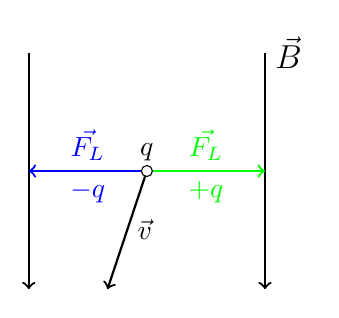
\begin{tikzpicture}
	\draw[->, thick] (0,0) -- (0,-3);
	\draw[->, thick] (3,0) node[right] {\large{$\vec{B}$}} -- (3,-3);

	\draw[->, thick, draw=green] (1.5,-1.5) -- (3,-1.5) node[above, midway, text=green] {$\vec{F_L}$} node[below, midway, text=green] {$+q$};
	\draw[->, thick, draw=blue] (1.5,-1.5) -- (0,-1.5) node[above, midway, text=blue] {$\vec{F_L}$} node[below, midway, text=blue] {$-q$};

	\draw[->, thick] (1.5,-1.5) -- (1,-3) node[right, midway] {$\vec{v}$};

	\draw[fill=white] (1.5,-1.5) circle (0.07) node[above] {$q$};
\end{tikzpicture}
%Code
\begin{lstlisting}[frame=single]
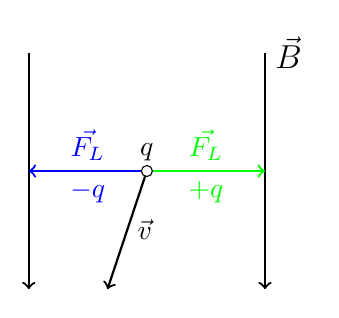
\begin{tikzpicture}
	\draw[->, thick] (0,0) -- (0,-3);
	\draw[->, thick] (3,0) node[right] {\large{$\vec{B}$}} -- (3,-3);

	\draw[->, thick, draw=green] (1.5,-1.5) -- (3,-1.5) node[above, midway, text=green] {$\vec{F_L}$} node[below, midway, text=green] {$+q$};
	\draw[->, thick, draw=blue] (1.5,-1.5) -- (0,-1.5) node[above, midway, text=blue] {$\vec{F_L}$} node[below, midway, text=blue] {$-q$};

	\draw[->, thick] (1.5,-1.5) -- (1,-3) node[right, midway] {$\vec{v}$};

	\draw[fill=white] (1.5,-1.5) circle (0.07) node[above] {$q$};
\end{tikzpicture}
\end{lstlisting}

\section{12.01.2009}
\subsection{12.01.2009-IMG-phys-1}
%Picture
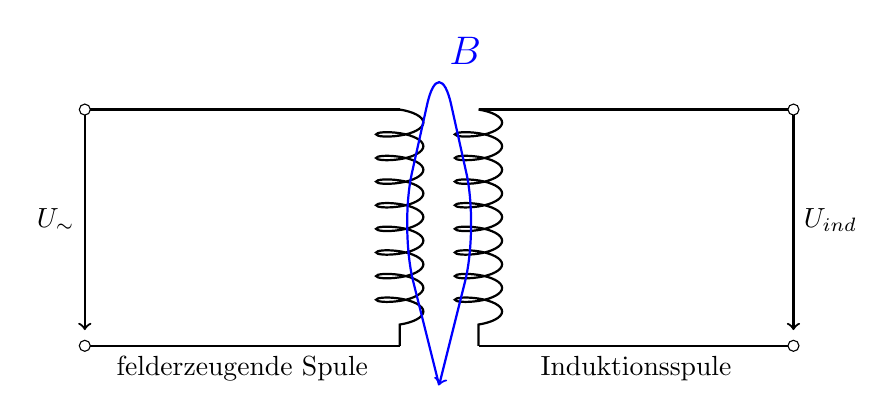
\begin{tikzpicture}[decoration={coil,aspect=0.3,segment length=3mm,amplitude=3mm}]

	%Linker Teil
	\draw[->, thick] (0,0) -- (0,-2.8) node[left, midway] {$U_{\sim}$};
	\draw[thick] (0,0) -- (4,0);
	\draw[thick] (4,-3) -- (0,-3) node[below, midway] {felderzeugende Spule};
	%Spule 1
	\draw[thick, decorate] (4,0) -- (4,-3);

	\draw[fill=white] (0,0) circle (0.07);
	\draw[fill=white] (0,-3) circle (0.07);

	%Rechter Teil
	\draw[thick] (5,0) -- (9,0);
	\draw[->, thick] (9,0) -- (9, -2.8) node[right, midway] {$U_{ind}$};
	\draw[thick] (5,-3) -- (9,-3) node[below, midway] {Induktionsspule};
	%Spule 2
	\draw[thick, decorate] (5,0) -- (5,-3);

	\draw[fill=white] (9,0) circle (0.07);
	\draw[fill=white] (9,-3) circle (0.07);

	\draw[thick, draw=blue, ->, rounded corners=20pt] (4.5,-3.5) -- (4,-1.5) -- (4.5,0.75) node[right, text=blue] {\Large{$B$}} -- (5,-1.5) -- (4.5,-3.5);
\end{tikzpicture}
%Code
\begin{lstlisting}[frame=single]
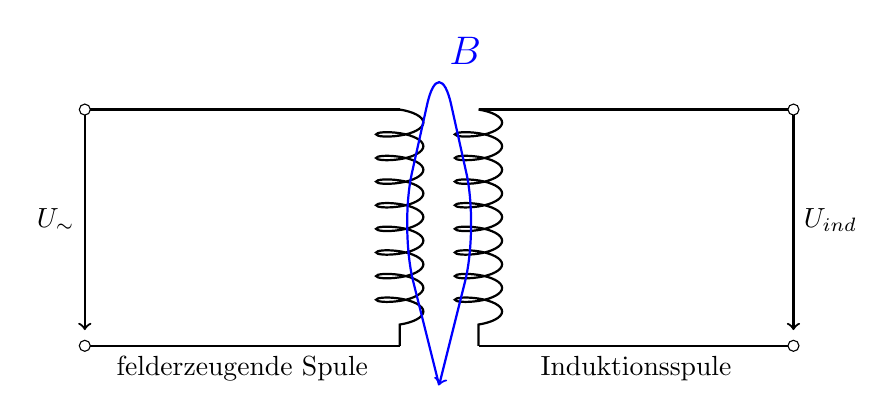
\begin{tikzpicture}[decoration={coil,aspect=0.3,segment length=3mm,amplitude=3mm}]

	%Linker Teil
	\draw[->, thick] (0,0) -- (0,-2.8) node[left, midway] {$U_{\sim}$};
	\draw[thick] (0,0) -- (4,0);
	\draw[thick] (4,-3) -- (0,-3) node[below, midway] {felderzeugende Spule};
	%Spule 1
	\draw[thick, decorate] (4,0) -- (4,-3);

	\draw[fill=white] (0,0) circle (0.07);
	\draw[fill=white] (0,-3) circle (0.07);

	%Rechter Teil
	\draw[thick] (5,0) -- (9,0);
	\draw[->, thick] (9,0) -- (9, -2.8) node[right, midway] {$U_{ind}$};
	\draw[thick] (5,-3) -- (9,-3) node[below, midway] {Induktionsspule};
	%Spule 2
	\draw[thick, decorate] (5,0) -- (5,-3);

	\draw[fill=white] (9,0) circle (0.07);
	\draw[fill=white] (9,-3) circle (0.07);

	\draw[thick, draw=blue, ->, rounded corners=20pt] (4.5,-3.5) -- (4,-1.5) -- (4.5,0.75) node[right, text=blue] {\Large{$B$}} -- (5,-1.5) -- (4.5,-3.5);
\end{tikzpicture}
\end{lstlisting}

\subsection{12.01.2009-IMG-phys-4}
%Picture
\begin{tikzpicture}
	\draw[->, thick] (0,0) node[left] {$B$} -- (0,3) node[left] {$U_N$};
	\draw[->, thick] (-0.2,1.5) node[left] {$I$} -- (5,1.5) node[below] {$t$};
	\draw (0,2.5) -- (5,2.5);
\end{tikzpicture}
%Code
\begin{lstlisting}[frame=single]
\begin{tikzpicture}
	\draw[->, thick] (0,0) node[left] {$B$} -- (0,3) node[left] {$U_N$};
	\draw[->, thick] (-0.2,1.5) node[left] {$I$} -- (5,1.5) node[below] {$t$};
	\draw (0,2.5) -- (5,2.5);
\end{tikzpicture}
\end{lstlisting}

\subsection{12.01.2009-IMG-phys-5}
%Picture
\begin{tikzpicture}
	\draw[->, thick] (0,0) -- (0,3);
	\draw[->, thick] (-0.2,1.5) node[left] {$0$} -- (5,1.5) node[below] {$t$} node[below, midway] {$U_{ind} > 0$};
\end{tikzpicture}
%Code
\begin{lstlisting}[frame=single]
\begin{tikzpicture}
	\draw[->, thick] (0,0) -- (0,3);
	\draw[->, thick] (-0.2,1.5) node[left] {$0$} -- (5,1.5) node[below] {$t$} node[below, midway] {$U_{ind} > 0$};
\end{tikzpicture}
\end{lstlisting}
